\documentclass{article}
\usepackage{graphicx} % Required for inserting images
\usepackage{amsmath}
\usepackage{minted}

\title{Differential Equations Coding Project}
\author{Cam Walter}
\date{April 24, 2024}

\begin{document}

\maketitle

\section*{Questions}

\begin{enumerate}
  \item
        \begin{enumerate}
          \item \begin{math}
                  f(x) = -5 + 0.5x^2 + x^5
                \end{math}
          \item The solution would not work, since we would need a degree 6
                polynomial now. This makes sense, since if we added a row to multiply,
                there would not be enough columns in A to match up with x's rows.
          \item \begin{math}
                  det(V)=0 \iff \exists x_i, x_j (x_i=x_j)
                \end{math}
          \item 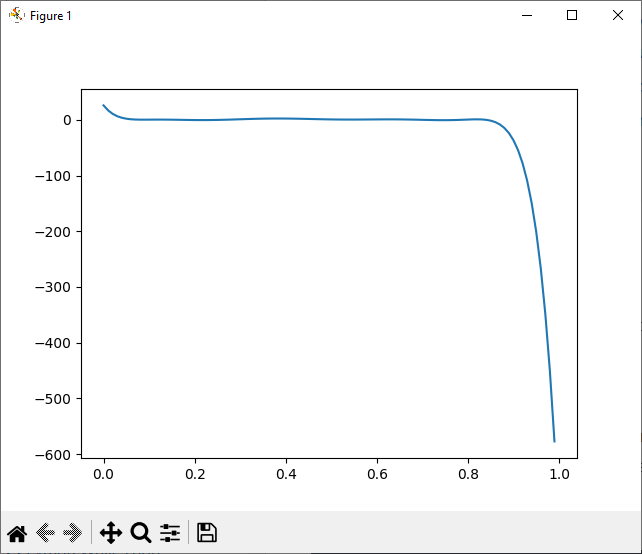
\includegraphics[width=\linewidth]{image.png}
          \item We can use spline interpretation to form a piecewise function
                comprised ofseveral small polynomials to make the graph much better
                reflect the data points.
        \end{enumerate}

  \item \begin{enumerate}
          \item
        \end{enumerate}
\end{enumerate}

\pagebreak

\section*{Code}
\inputminted{python3}{main.py}

\end{document}
